%----------------------------------------------------%
%                    INTRODUCCION                    %
%----------------------------------------------------%

\pagestyle{fancy}

\chapter{Introducción}
\label{introduccion}

Desde Aristóteles y su libro Segundos Analíticos \footnote{\href{https://docs.google.com/a/datik.es/file/d/0By4kcbi6MzzdUHhVQnUtcTNUdk0/view}{Órganon II de Aristóteles: Recopilación de obras Aristotélicas que incluye el libro Segundo Analíticos}} hasta Galileo, padre de la ciencia moderna, adalides del conocimiento han proclamado que un método de investigación basado en lo empírico y en la medición, sujeto a los principios específicos de las pruebas de razonamiento es el camino para conocer la verdad.\\

Hoy en día, época en la que los avances tecnológicos han posibilitado observar y medir de forma exhaustiva un gran abanico de fenómenos, la ingente cantidad de datos que se genera en el proceso es, a veces, intratable mediante las tecnologías convencionales, y por ende, es imposible extraer todo el conocimiento que atesoran. El problema, lejos de atenuarse, se acrecienta con el paso del tiempo. Estudios como el realizado por McKinsey Global Institute \footnote{\href{http://www.mckinsey.com/mgi/overview}{McKinsey Global Institute}} estiman que el volumen de datos que se genera crece un 40\% cada año y auguran que entre 2009 y 2020 se verá multiplicado por 44 \cite{nambiartowards}.\\

Por ello, en los últimos años ha irrumpido la necesidad de desarrollar nuevas metodologías y tecnologías que permitan procesar y extraer el conocimiento que fluye dentro del torrente informativo en la cual se encuentra sumergida la sociedad moderna, dando como resultado el nacimiento del Big Data\cite{manyika2011big}.\\

Empresas de renombre mundial, conscientes de los beneficios que les puede reportar en diferentes aspectos de su negocio, ya se han interesado en este fenómeno. De un estudio realizado entre los altos ejecutivos de las firmas que lideran el Wall Street se desprende que el 96\% tiene planeadas ciertas iniciativas relacionadas con el Big Data, y el 80\% ya tiene finalizada alguna \cite{bdes:2013}. 

\section{Contexto}
 
Datik Información Inteligente \footnote{\url{http://www.datik.es/}} es una empresa tecnológica perteneciente al Grupo Irizar \footnote{\url{http://www.irizar.com/irizar/}}  que desarrolla soluciones ITS destinadas a la gestión del trasporte, tanto ferroviario como por carretera y movilidad ciudadana.\\

Uno de los productos estrella de la entidad es el denominado iPanel, concentrador de  información que ofrece al operador de transporte servicios de valor añadido en la gestión de la información generada por su flota. El funcionamiento del servicio se puede resumir mediante la Figura \ref{fig:ipanel}:\\

\begin{figure}[h]
	\centering
	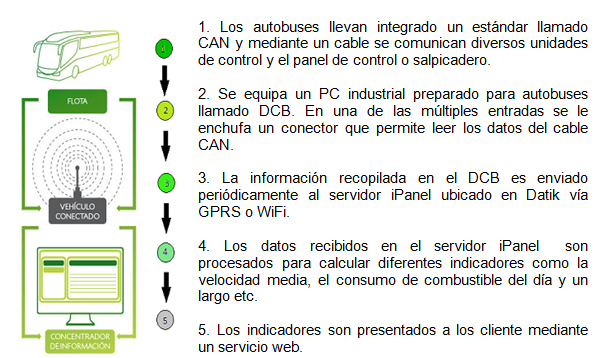
\includegraphics[width=1\textwidth]{Ilustraciones/ipanel_infraesctructure.png}
	\caption{Funcionamiento resumido de iPanel}
	\label{fig:ipanel}
\end{figure}

La incesante integración de nuevos vehículos en iPanel ha generado un crecimiento exponencial del número de registros almacenados en ciertas tablas MySQL. Aunque el volumen actual no llega a suponer riesgo alguno para el funcionamiento del servicio, Datik tiene identificados varios escenarios en los que la situación se podría revertir, causando graves problemas en el sistema.\\

Uno de los problemas, intrínseco a operar sobre una base de datos centralizada, es el riesgo de que ésta se convierta en cuello de botella. Al ser el punto donde todos los procesos confluyen, el bloqueo o la caída causada por uno de ellos puede afectar al resto. Para solventarlo, Datik ha optado por migrar su infraestructura a otra basada en Microservicios \cite{newman2015building}, esperando lograr el aislamiento total de los procesos que conforman sus servicios.\\ 

Otro problema es el referente al Cálculo de Indicadores: proceso de ejecución diaria que realiza operaciones aritméticas intensivas sobre datos almacenados en diversas tablas para después, agrupar los resultados en base a diferentes criterios. Siendo dichas tablas las que mayor crecimiento experimentan, el aumento del volumen de las mismas incrementa de forma desorbitada el tiempo necesario para finalizar el cálculo, pudiendo, en un futuro, llegar a tardar más de 24 horas y cancelar los indicadores que ofrecen información del último día.\\

El objetivo del presente proyecto es proponer una solución tecnológica que solvente permanentemente los problemas derivados de operar sobre volúmenes masivos de datos como en el caso del proceso Cálculo de Indicadores u otros similares que pudieran emerger en un futuro.\\

\section{Propuesta}

Tal y como se ha mencionado en apartados anteriores, la problemática que envuelve al Cálculo de Indicadores es originado por el incremento exponencial de datos que dicho proceso ha de tratar. No sería descabellado pensar que la solución pudiera pasar por escalar la máquina verticalmente y afinar la configuración de MySQL. No obstante, ambas mejoras son limitadas, mientras que el volumen de los datos seguirá en aumento de forma inexorable, volviendo, tarde o temprano, a tener que lidiar con los mismos problemas del principio.\\

Siendo imposible reconducir la situación usando las tecnologías tradicionales, en el presente proyecto se propone realizar un cambio de paradigma que implica migrar las tablas relacionadas con los indicadores a un modelo distribuido que posibilite escalar la infraestructura horizontalmente. A su vez, se sugiere dividir el problema en dos apartados, almacenamiento y procesado, dotando la infraestructura de tecnología adecuada para ofrecer una respuesta eficaz a cada una de las partes.\\

En cuanto a almacenamiento se refiere, teniendo en cuenta que los datos a tratar no presentan relación alguna con el resto de las entidades, se propone utilizar una base de datos no relacional. Dentro de la extensa gama de sistemas de almacenamiento NoSQL\footnote{\url{http://nosql-database.org/}} que existen hoy en día, se ha considerado que Apache Cassandra\cite{lakshman2010cassandra} es el idóneo para solventar este problema debido a que ofrece un ratio de escrituras por segundo sustancialmente superior en comparación a sus homólogos\cite{rabl2012solving}.

// Hablar de Apache Spark

// Hablar tambien de los datos

Analizando el escenario presentado, 

** Los datos con los cuales se hara a prueba no son de datik, por motivos de confidencialidad de cantidad

Apache Cassandra es una base de datos distribuida no-sql. Gracias a naturaleza distribuida ayuda a resolver, 

Funcionalidades nuevas que trabajan con videos etc



(testear las tecnologias con dataset publico, los datos de la empresa son confidenciales) Debido a la falta de datos se ha utilizado un dataset publico para emular las condiciones de futuro con las que se va a encontrar datik

\section{Organización del documento}

En esta memoria se ha documentado  el desarrollo de la herramienta \textbf{\textit{exerClick}}, dentro del Trabajo de Fin de Grado (TFG) del autor. En el documento se describe la propuesta, la planificación y gestión que esta lleva consigo, la implementación llevada a cabo y las conclusiones finales.\\

En este primer capítulo se ha introducido el problema a resolver y se ha explicado la propuesta presentada en este proyecto.\\

En el capítulo 2 se presenta el Documento de Objetivos de Proyecto (DOP). Este recoge el alcance y las fases y tareas del proyecto, el análisis de riesgos y el análisis de factibilidad.\\

Una vez en el capítulo 3 se explica la gestión llevada a cabo durante el proyecto. Se presentan las metodologías utilizadas: Metodologías Ágiles e InterMod (adaptada a las necesidades de este proyecto). A continuación se detallan cada una de las iteraciones llevadas a cabo (como parte de la metodología InterMod): duración, objetivos y tareas realizadas. Al final del capítulo se muestra la documentación asociada a las iteraciones y los objetivos, además del seguimiento de tiempo realizado.\\

A continuación, en el capítulo 4 se detalla el análisis de requisitos. Primero se detallan los requisitos no-funcionales y luego los funcionales (prototipos en papel llevados a cabo durante las primeras iteraciones que dan una visión global del proyecto).\\

En el capítulo 5 se explica el diseño e implementación llevados a cabo. Se comienza mostrando la estructura de documentos del proyecto, luego el diseño realizado en base al análisis de requisitos del capítulo 4 y finalmente una visión general de la implementación de la lógica de negocio.\\

Para finalizar, en el capítulo 6 se presentan las conclusiones, líneas futuras para el proyecto y las lecciones aprendidas.\\

Fuera de la estructura general de la memoria, tenemos la bibliografia y los apéndices. En estos últimos tenemos las actas de reuniones, las actas de pruebas y la vista de relaciones de la base de datos (de la parte utilizada o creada específicamente para el proyecto).\\